\section{Merging Diverse Plans into a TPN}
\label{generating: merging}
A naive merging approach for generating a TPN would be to create a single decision variable $v \in V$ corresponding to a choice 
between the $k$ obtained solutions. 
The structure of the TPN would then be a single decision at the
initial state, which is shared, and then the $k$ constituent plans running in parallel
up until they merge at the end of their path when reaching the terminal state which to is shared.
We denote this structure from now on as the \textit{naive TPN}. 
Although this approach defeats the purpose of having a flexible plan with choices, we would like to emphasize 
the fact that the naive TPN is attainable for any set of $k$ solutions. This means that no matter how big $k$ is 
or the length of each solution, we can always generate a functioning TPN to pass onward to Pike.
This by itself is already good news and provides our process with a degree of safety as a first step. 
    
The technique we describe here starts with the aforementioned naive TPN, but then looks for opportunities to merge additional time points.
It is convenient to think of a TPN as a graph where time points are nodes connected by constraints (edges).
By merging time points, additional solutions can be created, as demonstrated by the example in Figure \ref{fig:add_plans_from_merge}.


\begin{figure}
\centering
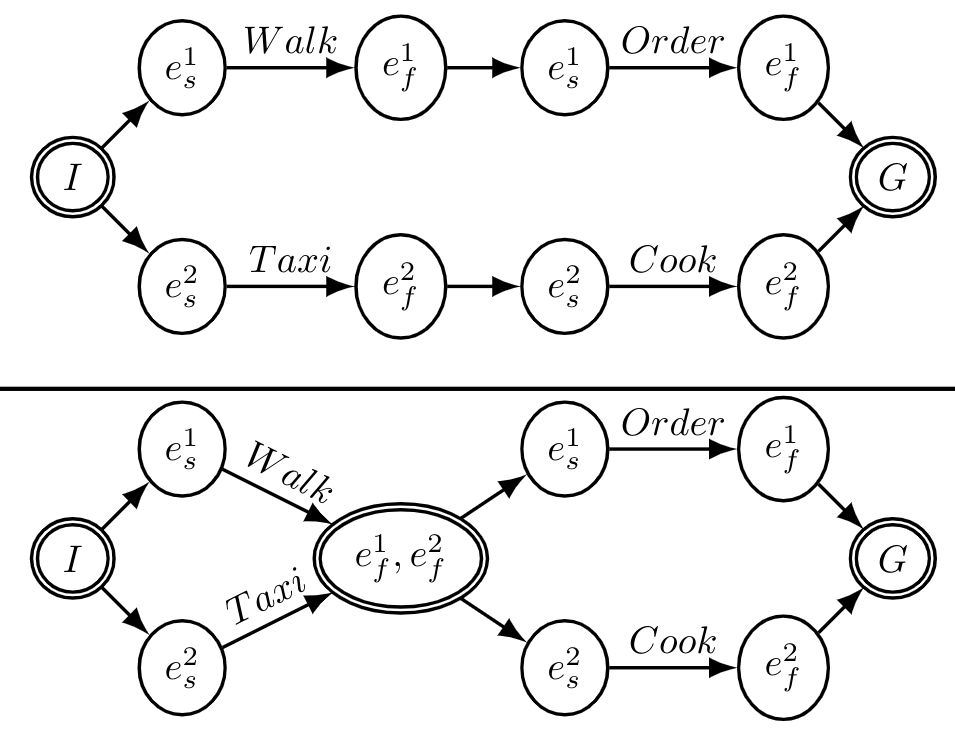
\includegraphics[width=0.8\textwidth]{graphics/merge.png}
 \label{fig:add_plans_from_merge}
\caption{Additional paths in the graph are created as a result of a merge.} 
\end{figure}

% \begin{figure}%[H]
%     \centering
%     \begin{minipage}[t]{0.5\textwidth}  \centering
%         \begin{tikzpicture}[thick,scale=0.9, every node/.style={transform shape}]
%             % x node set with absolute coordinates
%             \node[state, accepting] (a) at (0,-1) {$I$};
%             \node[state] (b) at (1,0) {$e^1_s$};
%             \node[state] (c) at (3,0) {$e^1_f$};
%             \node[state] (d) at (4.5,0) {$e^1_s$};
%             \node[state] (e) at (6.5,0) {$e^1_f$};
%             \node[state] (f) at (1,-2) {$e^2_s$};
%             \node[state] (g) at (3,-2) {$e^2_f$};
%             \node[state] (h) at (4.5,-2) {$e^2_s$};  
%             \node[state] (i) at (6.5,-2) {$e^2_f$};
%             \node[state, accepting] (j) at (7.5,-1) {$G$};
%             % Directed edge
%             \draw (a) edge (b);
%             \draw (b) edge node[pos=0.5, sloped, above] {$Walk$} (c);
%             \draw (c) edge  (d);
%             \draw (d) edge node {$Order$} (e);
%             \draw (a) edge  (f);
%             \draw (f) edge node[pos=0.5, sloped, above] {$Taxi$} (g);
%             \draw (g) edge  (h);
%             \draw (h) edge node {$Cook$} (i);
%             \draw (i) edge (j);
%             \draw (e) edge (j);
%         \end{tikzpicture}
%     \end{minipage}
%     \centerline {\rule{.8\linewidth}{1pt}}
%     \begin{minipage}[t]{0.5\textwidth} \centering
%         \begin{tikzpicture}[thick,scale=0.9, every node/.style={transform shape}]
%             % x node set with absolute coordinates
%             \node[state, accepting] (a) at (0,-1) {$I$};
%             \node[state] (b) at (1,0) {$e^1_s$};
%             \node[state] (d) at (4.5,0) {$e^1_s$};
%             \node[state] (e) at (6.5,0) {$e^1_f$};
%             \node[state] (f) at (1,-2) {$e^2_s$};
%             \node[state] (h) at (4.5,-2) {$e^2_s$};  
%             \node[state] (i) at (6.5,-2) {$e^2_f$};
%             \node[state, accepting] (m) at (3,-1) {$e^1_f,e^2_f$};
%             \node[state, accepting] (j) at (7.5,-1) {$G$};
%             % Directed edge
%             \draw (a) edge (b);
%             \draw (b) edge node[pos=0.5, sloped, above] {$Walk$} (m);
%             \draw (m) edge  (d);
%             \draw (d) edge node[pos=0.5, sloped, above] {$Order$} (e);
%             \draw (a) edge  (f);
%             \draw (f) edge node[pos=0.5, sloped, above] {$Taxi$} (m);
%             \draw (m) edge  (h);
%             \draw (h) edge node[pos=0.5, sloped, above] {$Cook$} (i);
%             \draw (i) edge (j);
%             \draw (e) edge (j);
%         \end{tikzpicture}
%     \end{minipage}
%     \caption{Additional paths in the graph are created as a result of a merge. Choice time points are depicted with double circles.\\
%     \textbf{Top:} Two separate plans, number of possible paths: 2. \\
%     \textbf{Bottom:} Two merged plans, number of possible paths: 4.}
%     \label{fig:add_plans_from_merge}
%     \vspace{-4mm}
% \end{figure}


\begin{tcolorbox}[colback=red!5!white,colframe=red!75!black]
  \textit{Returning to our running example, let us consider the case where our robot, Rob, has conceived two constituent plans
   shown in a \textit{naive} TPN fashion at the top of Figure \ref{fig:add_plans_from_merge}.
   The plans are: $i$) walk home and then order in, or $ii$) take a taxi home and then cook.
   By merging a time point between the two paths, we obtain a new TPN, as portrayed in the lower section of the Figure, which yields 2 
   new solutions: walking home and then cooking, and taking a taxi home and then ordering in.
  }
\end{tcolorbox}


We next describe how we choose which time points from the naive TPN to merge.


\subsubsection{Merging Time Points in the TPN} 
While it is theoretically possible to merge any two time points in the TPN, it is likely a bad idea to merge two random time points. 

Some intuitive approaches include \textit{i)} comparing the underlying PDDL states of time points and \textit{ii)} comparing ordered sequences of activities originating from time points.
Unfortunately, both techniques fall short of accounting for important merges possibilities we wish to obtain. We showcase one of these approaches bellow:\\
\\
\textbf{State Space Comparison:} This approach imposes that for two time points to be merged, they must hold the same set of fact literals $F$. Although this constraint does ensure that time points that are chosen for merge can indeed be merged, it is too restrictive.\\
\begin{tcolorbox}[colback=red!5!white,colframe=red!75!black]
  \textit{Consider the merge witnessed in Figure \ref{fig:add_plans_from_merge}. The time points merged denoted the end of the activities whose purpose was to get Rob home. Once home, we can assume that the underlying PDDL states of $e^1_f$ and $e^2_f$ are similar and therefore this merge is plausible.\\
  Now consider a similar scenario with one key difference --- there exists a literal indicating the amount of money Rob has spent.
  Given that walking is free and a taxi costs money, we can expect that this state space comparison would rule out $e^1_f$ and $e^2_f$ as applicable for a merge.
    }
\end{tcolorbox}
This example shows how sensitive this method can be to the way each domain was constructed. 
Intuition would suggest that the solution to this issue is in locating the minimal set of literals that are of importance and only comparing those instead of all. This adjustment would work however the domain independent nature of automated planning makes finding this set of literals a nontrivial problem.
\\ \\
Thus we suggest a method to determine whether two time points should be merged based on the validity of the solutions originating from their merge.
We introduce the {\em compatibility} attribute of two IHs. We define compatibility based on IHs as opposed to time points as the latter can change when merging time points in the TPN while the former remains a static property of the TPSs of the original diverse solutions.
We define two notions of compatibility:
\begin{definition}[\textbf{IHs Compatibility}]
Given a pair of IHs $a_1,a_2$ from TPSs $\pi_i,\pi_j$ respectively, 
let $s_{a_1},s_{a_2}$ be 
the underlying PDDL state after these IHs occurred in $\pi_i,\pi_j$, respectively, and let their corresponding TPS suffixes be $\Sigma^{\pi_i}_{a_1}, \Sigma^{\pi_j}_{a_2}$.
$a_1,a_2$ are:
\begin{itemize}
    \item \textbf{Fully compatible} iff $G \subseteq T(s_{a_1},\Sigma^{\pi_j}_{a_2}) \; and \; G \subseteq T(s_{a_2},\Sigma^{\pi_i}_{a_1})$
    \item  \textbf{Semi compatible} iff $G \subseteq T(s_{a_1},\Sigma^{\pi_j}_{a_2}) \;  or \;  G \subseteq T(s_{a_2},\Sigma^{\pi_i}_{a_1})$
\end{itemize}
\end{definition}

In other words two IHs $a_1,a_2$ are Fully Compatible if we can execute the TPS suffix of each $\pi$ from the other's current state $s_a$ and achieve the goal, while two IHs $a_1,a_2$ are merely Semi Compatible if we can execute at least one of the TPS suffixes from the other's current state $s_a$ and achieve the goal.

We denote the set containing all such compatible pairs as $\MergeSet$. Since $\MergeSet$ is static, we can efficiently compute it once at the beginning of the process.
Each pair of compatible IHs $\{a_1,a_2\} \in \MergeSet$ is an operation $m$ corresponding to a merge we can perform on the TPN time points. 

From now on, we will restrict our attention to applying only merges between pairs contained in $\MergeSet$ to the TPN. While this limits the space of possible TPNs, it also reduces the complexity of the problem to a manageable size.
\\ \\  
Merging two time points in the TPN outputs a single new time point. This new time point must account for all IHs involved in the merge (recall that a time point may consist of multiple IHs). Therefore the merging of two time points is an operation between sets of IHs. Consider the 2-step merging sequence to the naive TPN $m(a_1,a_2),m(a_2,a_3)$. The first merge operation creates a new time point $e_{new}$. The second merge operation is now $m(e_{new},a_3)=m(\{a_1,a_2\},a_3)$.

This scenario raises questions about the compatibility attribute as it applies to sets of IHs. We can define different transitivity notions when merging in order to experiment with this concept and widen or narrow our solution space.
\begin{definition}[\textbf{Merge Transitivity}] 
    We define two notions of transitivity for when we allow merges to be made.
    Formally, a merge between time points $e_1,e_2$ is applicable iff:
    \begin{itemize}
        \item \textbf{Strict}: $\forall a_i \in e_1 \wedge \forall a_j \in e_2:   m\{a_i,a_j\} \in \MergeSet$ 
        \item \textbf{Loose}: $\exists a_i \in e_1 \wedge \exists a_j \in e_2: m\{a_i,a_j\} \in \MergeSet$
    \end{itemize}
\end{definition}

We have not limited ourselves to generating TPNs with only valid solutions as the TPN executive (Pike) incorporates the ability to avoid making combinations of choices that lead to infeasible paths \cite{levine2018watching}.
